\chapter{Introduction\label{chap:introduction}}

\section{Small molecule drug design\label{sec:drug-design}} The discovery of novel drugs has
contributed significantly to the improvement of human health and well-being. There is a continous
demand for new drugs, in order to expand the range of treatable diseases, to improve the efficacy of
existing treatments and to respond to the emergence of new diseases.

Small molecule drugs are the major kind of medicines in use, constituting as much as 90\% of global
sales \citep{makurvetBiologicsVsSmall2021}. Small molecules are usually defined as molecules with a
molecular weight of less than 900 Da. These molecules often are orally available, have good
pharmacokinetic properties and can be synthesized in a cost-effective manner \citep{todo}.

For a small molecule to be a viable drug candidate it needs to fulfill a whole range of properties
\citep{todo}:
\begin{itemize}
      \item \textbf{On-target activity:} The molecule needs to be active against the desired target
            in order for it to show the desired therapeutic effect. On a molecular level this means
            that the molecule needs to bind to the target and modulate its activity in the desired
            way.
      \item \textbf{Pharmacokinetics:} The molecule must have favourable pharmacokinetic properties
            such as adsorption, distribution, metabolism and excretion (ADME). ADME determine how
            the molecule is absorbed into the body, how it is distributed in the body, how it is
            metabolized and how it is excreted from the body. These properties are crucial for the
            molecule to reach the target in the body and to be metabolized in a safe manner and to
            finally be excreted from the body.
      \item \textbf{Toxicity:}  The absence of toxic effects is crucial, as the molecule must be
            well-tolerated and devoid of any potential harmful side effects. Toxicity can be caused
            by a range of factors, including off-target interactions, metabolic byproducts or
            allergies.
      \item \textbf{Specificity:}  The molecule should exhibit high specificity, selectively
            interacting with the intended target while minimizing undesirable off-target
            interactions. Off-target binding can lead to adverse side effects and potentially
            compromise the drug's safety and efficacy profile.
      \item \textbf{Synthesizability:} The molecule must be synthesizable in a cost-effective manner
            to be practically useful.
      \item \textbf{Patentability:} The molecule must be novel and not infringe on any existing
            patents. While in general this is not needed for a drug to work, this constitutes a
            significant issue in practice.
\end{itemize}

The main challenge in drug discovery is to find a molecule that fulfills all these mentioned
properties. The development of a new drug is a complex and expensive process, which can take up to
10--15 years and costs up to 3 billion USD \citep{todo}.


\subsection{The drug discovery pipeline}
The drug discovery process is usually divided into several stages depicted in
\Cref{fig:drug-discovery-pipeline} and described below.
\begin{figure}
      \centering
      \includegraphics[width=\textwidth]{figures/drug-discovery-pipeline.pdf}
      \caption{The drug discovery pipeline starts with the identification of a biological target.
            Once a target is identified, readily available molecules are screened for their activity
            against the target in high-throughput screening. Promising hits are then modified and
            optimized to lead compounds. These lead compounds are then further optimized and tested
            in preclinical. Finally, the most promising candidates are tested in clinical trials and
            eventually approved by regulatory agencies. The stages in the blue box are highly
            amenable to machine learning and computational methods and are the focus of this
            thesis.\label{fig:drug-discovery-pipeline}}
\end{figure}
\begin{itemize}
      \item \textbf{Target identification:} The drug discovery process starts with the
            identification of a biological target, which is a molecule or a protein that is involved
            in a disease process.
      \item \textbf{Hit discovery:} In the hit discovery stage molecules are screened for their
            activity against the target in high-throughput screening (HTS). These lab experiments,
            often referred to as assays, are used to measure the activity of the molecules against
            the target in vitro. This stage results in a set of so called hits, which are molecules
            that show activity against the target.
      \item \textbf{Hit-to-lead:} Promising hits are then modified and optimized to lead compounds.
            In this stage, the optimization is primarily focused on improving the activity of the
            molecule against the target. This is usually done in a DMTA (Design-Make-Test-Analyze)
            cycle, where the molecule is designed, synthesized, tested in vitro. The results are
            then analyzed and the cycle continues until a satisfactory lead compound is found.
      \item \textbf{Lead optimization:} The lead compounds are then further optimized to improve
            their properties, such as pharmacokinetics, toxicity or specificity. This is usually
            done in a DMTA cycle as in the hit-to-lead stage and also involves the synthesis and
            testing of the molecules in vitro.
      \item \textbf{Preclinical development:} The most promising candidates are then tested in
            preclinical studies. These studies are usually done in animals and are used to assess
            the safety and efficacy of the drug candidate in vivo.
      \item \textbf{Clinical trials:} Finally, the candidates that pass the preclinical studies are
            tested in humans in clinical trials. These are usually divided into three phases, where
            the safety and efficacy of the drug are tested in increasing numbers of patients. Phase
            I trials are mainly focused on the safety of the drug, Phase II trials are focused on
            the efficacy of the drug and Phase III trials are focused on the safety and efficacy of
            the drug in a larger population.
      \item \textbf{Regulatory approval:} The final stage is the regulatory approval, where the drug
            is approved by regulatory agencies such as the FDA in the US or the EMA in Europe.
\end{itemize}

The general strategy of this stagewise approach is to reduce the uncertainty about the usefulness of
a molecule at each stage. The earlier stages are usually cheaper and faster, but have higher
uncertainty about the clinical success of the molecule. The later stages are more expensive and
slower, but provide better information about the success chances of a molecule \citep{todo}.

The success rates of clinical trials are low, with only about 10\% of drugs that enter clinical
trials eventually being approved by regulatory agencies More specifically, the success rates in
Phase I/II/III and the final regulatory approval are 63\%, 31\%, 58\% and 85\% respectively
\citep{mullardParsingClinicalSuccess2016}. This translates to 63\%, 19.5\%, 11.3\% and 9.6\% of
projects that make it to the respective stages.

\subsection{The Design-Make-Test-Analyze cycle}
\begin{figure}
      \centering
      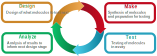
\includegraphics[width=\textwidth]{figures/dmta_cycle.pdf}
      \caption{The DMTA cycle}
\end{figure}
% Todo: expand this a little bit
The hit discovery, hit-to-lead and lead optimization stages (blue box in
\Cref{fig:drug-discovery-pipeline}) usually operate in an iterative manner, resulting in a cycle of
choosing molecules to be tested, synthesizing them, testing them in laboratory experiments and
analyzing the results to guide the selection of the next molecule to be tested. This cycle is
usually referred to as the \ac{DMTA}-cycle:
\begin{itemize}
      \item \textbf{Design:} Under consideration of previous experimental results, the molecules to
            be tested are designed. The design generally aims to optimize the desired properties of
            the molecule, but also aims to maximize the information gained from the experiment. This
            stage often relies on computational methods to predict the properties of the molecules.
      \item \textbf{Make:} The designed molecules are then synthesized in the laboratory. This step
            requires a synthesis plan that outlines the steps needed to synthesize the molecule.
      \item \textbf{Test:} The synthesized molecules are then tested in laboratory experiments to
            measure the properties of interest.
      \item \textbf{Analyze:} The results of the experiments are then analyzed. involves the
            evaluation of the performance of the prediction models used in the design phase. The
            results of the analysis are then used to guide the design of the next molecule to be
            tested.
\end{itemize}

Computational methods are widely used throughout the DMTA cycle. One of the most important
applications of computational methods in drug discovery is the prediction of the properties of
molecules. These properties can range from the activity of a molecule against a target, to its
pharmacokinetic properties, to its toxicity. These \ac{QSPR} models are used to predict the
properties of molecules in the design phase, to guide the selection of molecules to be tested.

Recent years have seen a surge of interest in generative models for drug discovery, expanding the
capabilities of computer-aided drug design to tasks that produce molecular structures as outputs.
This thesis focuses on two critical applications: de novo drug design, which aims to discover
molecules with desired property profiles, and computer-aided synthesis planning, which seeks to
determine viable synthesis routes for molecules of interest. By harnessing the power of generative
models in these areas, we aim to accelerate the drug discovery process and pave the way for more
efficient development of potential new therapies.

\section{Generative models in drug discovery}
\subsection{Molecular Representations}
\begin{figure}
      \centering
      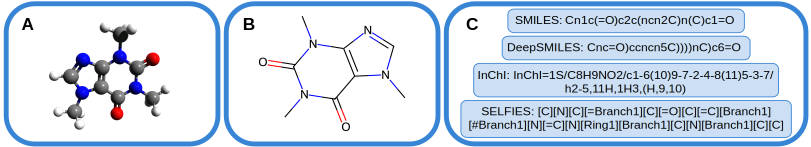
\includegraphics[width=\textwidth]{figures/representations/representations.pdf}
      \caption{Different ways to represent molecules. The molecule shown is caffeine \textbf{A:}
            Different 1D representations of a molecule. SMILES is an established line notation for
            molecules. DeepSmiles enables easier generation of molecules by getting rid of pair
            brackets and ring numbers. SELFIES guarantees that a sequence of tokens parses into a
            valid molecule. \textbf{B:} 2D graph representation of a molecule. The nodes represent
            atoms and the edges represent bonds. \textbf{C:} 3D structure of a molecule. The atoms
            are positioned in 3D space. The positions of these atoms can change as some bonds are
            allow rotations. Source of the 3D structure:
            \citep{EnglishCaffeine3D2010}.\label{fig:molecular-graph}}
      % TODO: add adjacency matrix representation
\end{figure}
Molecules, though fundamentally complex quantum mechanical entities, can be represented through
various simplified models for practical purposes. The most common representation depicts molecules
as graphs, where atoms are nodes and chemical bonds are edges. This graph structure captures the
molecule's connectivity, which defines its identity. Additional properties such as atom type,
charge, or chirality are incorporated as features of the nodes and edges.
%TODO: change letter
Figure \ref{fig:molecular-graph}b shows a graph representation of caffeine. While this representation
doesn't capture the full quantum complexity, it provides a stable and practical framework for
understanding and working with molecular structures in many scientific and computational contexts.

Molecular graphs can be linearized into one-dimensional character sequences, known as line
notations. Examples include INCHI \citep{hellerInChIIUPACInternational2015} and SMILES (Simplified
Molecular Input Line Entry System) \citep{weiningerSMILESChemicalLanguage1988}. SMILES strings have
proven particularly valuable for generative models, as they are easily processed by sequence-based
models like recurrent neural networks (RNNs) and transformers \citep{vaswaniAttentionAllYou2017}.
Several extensions to SMILES have been proposed to make them more amenable for use in
machine learning models. DeepSmiles \citep{oboyleDeepSMILESAdaptationSMILES2018} attempted
to make it easier to generate syntactically valid molecules, by changing the notation of
branches and ring closures. SELFIES \citep{krennSELFIESFutureMolecular2022} provide a
representation of molecules in which any sequence of tokens parses into a valid molecule.
SAFE \citep{noutahiGottaBeSAFE2023} provides a representation of molecules in which the
substructures are represented by contiguous regions of a SMILES string.

Molecules can be represented in various complex forms beyond simple graphs and strings.
Three-dimensional structures provide a spatial description of a molecule, detailing atomic positions
in 3D space along with information about atom types and bonds. The most comprehensive representation
is the quantum mechanical wavefunction, which captures the full complexity of molecular behavior.
While these more sophisticated representations are valuable for modeling a wide range of molecular
properties and interactions, but are not covered in the rest of this thesis.

\subsection{Generation strategies}
\paragraph{Sequence-based autoregressive models} constitute one of the most popular approaches for
generating molecules. Early work by \citep{seglerGeneratingFocusedMolecule2018} and
\citep{gomez-bombarelliAutomaticChemicalDesign2018} used recurrent neural networks (RNNs) to
generate molecules in SMILES format. Auto-regressive modelling is based on the idea of generating a
molecule by iteratively predicting the next characters of the SMILES string given the preciding
characters. The likelihood is thus modelled by $p(x) = \prod_{i=0}^n p(x_i | x_{1:i-1})$. This
approach has since been popular and there has been work on string-based representations more
suitable to generation
\citep{oboyleDeepSMILESAdaptationSMILES2018,krennSelfReferencingEmbeddedStrings2020}, parsing the
molecules into specialized data structures
\citep{kusnerGrammarVariationalAutoencoder2017,jinJunctionTreeVariational2018} and using other
architectures such as transformers \citep{vaswaniAttentionAllYou2017,noutahiGottaBeSAFE2023,schwallerMolecularTransformerModel2019,bagalMolGPTMolecularGeneration2022,mazuzMoleculeGenerationUsing2023}.

\paragraph{Graph-based autoregressive models} generate molecules in graph-based
representations. In this case the model generates the molecular graph by iteratively adding nodes
and edges to the graph. The model can be trained in a similar manner to the string-based models, by
predicting the next node or edge given the current state of the graph. However, the specification of
possible actions is more complex than in the 1D case as there is no natural ordering of the
nodes and edges in the graph \citep{cohen-karlikOvercomingOrderAutoregressive2024,youGraphConvolutionalPolicy2019}.

\paragraph{One-shot methods} are a class of models that generate molecules in one step, without the
need for an iterative generation process. These models generate an adjacency matrix and node feature
vector of a molecule in a single step. This is usually done by first generating a continous version
of the molecule and then discretizing it to a valid molecule \citep{decaoMolGANImplicitGenerative2018,madhawaGraphNVPInvertibleFlow2019,kadurinCornucopiaMeaningfulLeads2016}.

% https://www.frontiersin.org/journals/hematology/articles/10.3389/frhem.2024.1305741/full#h4
\paragraph{Rule-based models} generate molecules by applying a set of pre-defined graph transformation rules to
combine molecular fragments. The BRICS \citep{degenArtCompilingUsing2008} method provides a set of
molecular fragments and rules how to meaningfully combine them. This enables the generation of new
molecules by combining these fragments. DOGS \citep{hartenfellerDOGSReactionDrivenNovo2012}
generates molecules by applying a set of chemical reaction rules to a set of starting molecules,
which has the advantage of biasing generation towards synthesizable molecules.\@
\citet{jensenGraphbasedGeneticAlgorithm2019} defines graph mutation and crossover operations to
generate new molecules. These models allow the generation of molecules that are chemically valid, or
resemble known ``reasonable'' molecules.


\subsection{Distribution-learning}
% Whats distribution learning
Distribution-learning is a fundamental application of generative models in drug design. Its
objective is to create a model that accurately captures the distribution of molecules within a
dataset. Formally, the model learns a distribution $q(x)$ that approximates the true distribution
$p(x)$ of molecules. This approach enables the model to grasp both the syntax and semantics of the
molecules in the training set. As a self-supervised learning task, it allows models to leverage
large datasets. The resulting models serve two main purposes: they can expand virtual libraries and,
more crucially, act as a foundation for other applications such as goal-directed generation, which
we will explore in the subsequent section.

% \begin{align} \mathcal{L} = - \mathbb{E}_{x \sim p(x)} \log q(x). \end{align}
In recent years there has been a surge in interest distribution-learning models based on deep neural
networks. Many architectures and training strategies originally proposed for text and image
generation have been adapted and specialized to generate molecules. While all of them aim to
approximate $p(x)$, they differ in the way they model the distribution and the choice of molecular
representation.

\paragraph{Autoregressive models} can be directly trained using a maximum likelihood approach by
minimizing the cross entropy or \ac{NLL} of the training data
\begin{align}
      \mathcal{L} = - \mathbb{E}_{x \sim p(x)} \log q(x) \approx - \frac{1}{N} \sum_{i=1}^N \log q(x_i),
\end{align}
where $q(x)$ is the model distribution and $p(x)$ is the true distribution of the data. These models
are explicit density models, as the likelihood for a given molecule can be calculated exactly.
Autoregressive models form the backbone of many generative models in drug discovery
\citep{gomez-bombarelliAutomaticChemicalDesign2018,seglerGeneratingFocusedMolecule2018,olivecronaMolecularDenovoDesign2017,guoAugmentedMemoryCapitalizing2023,thomasAugmentedHillClimbIncreases2022,jaquesSequenceTutorConservative2016,cohen-karlikOvercomingOrderAutoregressive2024,}

\paragraph{Variational autoencoders} (VAEs) \citep{kingmaAutoEncodingVariationalBayes2013} generate molecules by first
sampling from a simple latent distribution $p(z)$, and then mapping the samples to molecular space
via a probabilistic decoder network $p(x|z)$. To make training tractable a second network, the
encoder network $q(z|x)$ is used to map the data to the latent space. The model is then trained to
maximize the evidence lower bound (ELBO) of the data
\begin{align}
      \log p(x) \geq \mathbb{E}_{q(z|x)}[\log p(x|z)] - \text{KL}(q(z|x) || p(z)),
\end{align}
where KL is the Kullback-Leibler divergence. This model has the advantage of providing a continuous
latent space, which can be used to interpolate between molecules and allows to run continuous
optimization algorithms in latent space. VAEs belong in the class of approximate density model, as
the likelihood of a given molecule can be calculated only approximately via monte carlo sampling.

% moflow, graphnvp (has nice discussion on one-shot generation)
\paragraph{Generative flows} \citep{rezendeVariationalInferenceNormalizing2016} are based on the idea of learning a bijective mapping between molecular
space and a latent space. Generative flows transform from a simple distribution $p(z)$ in latent space
to a distribution in chemical space, p(x), via a bijective mapping $G: z \rightarrow x$.
The likelihood of the training data can then be directly calculated and optimized
via the change of variables formula:
\begin{align}
      p(x) = p(z) \left| \det \frac{\partial G}{\partial z} \right|.
\end{align}
Originally generative flows have been proposed for continuous data, but have been adapted to
discrete data such as molecules by using a continuous relaxation of the molecule
\citep{madhawaGraphNVPInvertibleFlow2019}. These models also belong to the class of explicit density
models, as the likelihood of a given molecule can be calculated exactly.

% molgan
\textbf{Generative adversarial networks} (GANs) \citep{goodfellowGenerativeAdversarialNetworks2014}
are latent space models that map a simple distribution in latent space to molecular space, but rely
on a game-theoretic approach to training. A generator network is trained to generate data, which is
then fed to a discriminator network. The two networks then engage in a minimax game, where the
discriminator tries is trained to distinguish between real and generated data, while the generator
is trained to fool the discriminator.\@ \acp{GAN} are implicit density methods as calculating the
likelihood of a given molecule is not tractable.


\begin{figure}
      \centering
      \includegraphics[width=\textwidth]{./figures/goal_directed_cycle_and_virtual_screening.pdf}
      \caption{Comparison of goal-directed generative models and virtual screening. Goal-directed
            generation proceeds in a loop where already scored molecules inform what molecules to
            test next. Virtual screening proceeds in a linear fashion, where the molecules to be
            tested are determined beforehand. }
\end{figure}


\subsection{Goal-directed molecule generation\label{sec:goaldirected}}
Goal-directed molecule generation \citep{schneiderNovoMolecularDesign2013} is a computational
approach for automatically designing molecules with desired property profiles. Goal-directed
generation expands upon \ac{VS}, a method in which a library of molecules is ranked according to the
output of a \ac{QSPR} model.\ \citet{waltersVirtualChemicalLibraries2019} estimates that
approximately $10^{13}$ molecules can be routinely tested in a \ac{VS} experiment. While this number
can vary significantly depending on the computational cost of running the \ac{QSPR} model, it is
dwarfed by the size of drug-like chemical space, which is estimated to contain between $10^{30}$ and
$10^{60}$ molecules \citep{waltersVirtualChemicalLibraries2019,ruddigkeitEnumeration166Billion2012}.
Consequently, \ac{VS} is limited to exploring only a small fraction of chemical space and cannot
fully leverage the vast number of possible candidates that drug-like chemical space offers.

% How does DNDD help
Goal-directed generators address this limitation of \ac{VS} by focusing the search on the most
relevant parts of chemical space. In contrast to the random search approach taken by \ac{VS},
goal-directed generators act more like optimizers that are able to efficiently locate maxima. This
is achieved by an iterative process in which a model generates a set of molecules, which are then
scored by a \ac{QSPR} model. These scores are then used to update the model, shifting the sampling
distribution to regions of chemical space with higher scores.

Recently, there has been a surge of deep learning-based goal-directed generators
\citep{eltonDeepLearningMolecular2019,sanchez-lengelingInverseMolecularDesign2018,duMachineLearningaidedGenerative2024}.
A multitude of different models have been proposed, which are based on a variety of neural network
architectures, training strategies and molecular representations. These methods augment traditional
rule-based generation approaches that have been combined with graph search and evolutionary
algorithms. \citep{schneiderComputerbasedNovoDesign2005,schneiderNovoMolecularDesign2013}. The new
wave of deep-learning methods has shown great promise in generating novel molecules with desired
property profiles and have been used in a variety of applications, such as the design of new drugs,
materials or catalysts \citep{todo}.

Some of the most commonly used approaches to goal-directed molecular generation are:
\begin{itemize}
      \item \textbf{Hill-climbing}
            \citep{seglerGeneratingFocusedMolecule2018,xieMARSMarkovMolecular2021,thomasAugmentedHillClimbIncreases2022}
            is a simple optimization algorithm that relies on an underlying distribution-learning model.
            Molecules are sampled from the model's learned distribution and their scores are evaluated.
            The model is then retrained on the top-scoring molecules and the process is repeated.
      \item \textbf{Reinforcement learning} uses the molecule scores as a reward signal to update
            the model distribution. This is commonly via methods based on the REINFORCE algorithm
            \citep{williamsSimpleStatisticalGradientfollowing1992} which allows to update the model
            distribution in a way that increases expected scores of the generated molecules
            \citep{olivecronaMolecularDenovoDesign2017,thomasAugmentedHillClimbIncreases2022,youGraphConvolutionalPolicy2019,guoAugmentedMemoryCapitalizing2023}.
      \item \textbf{Genetic algorithms} transform an initial population of molecules by applying
            mutations and crossovers. The molecules are then evaluated and the best ones are
            selected for the next generation. Applying this process iteratively leads to a
            population of high-scoring molecules \citep{jensenGraphbasedGeneticAlgorithm2019,nigamGenerativeModelsSuperfast2021,yoshikawaPopulationbasedNovoMolecule2018}
      \item \textbf{Tree search} builds a tree of possible molecules by recursively applying a set
            of rules to to the current molecules. Molecules with higher scores are more likely to be
            expanded further \citep{yangChemTSEfficientPython2017,jensenGraphbasedGeneticAlgorithm2019}
      \item \textbf{Continuous optimization} employ classical optimization algorithms in the continuous
            latent space of (variational) autoencoders
            \citep{winterEfficientMultiobjectiveMolecular2019,gomez-bombarelliAutomaticChemicalDesign2018,kusnerGrammarVariationalAutoencoder2017}
            or generative flows \citep{madhawaGraphNVPInvertibleFlow2019}.
      \item \textbf{Generative Flow Networks} \citep{bengioFlowNetworkBased2021} aim to generate
            molecules with probability proportional to their score. This method relies on an
            iterative generation process and models chemical space as a directed acyclic graph, with
            nodes being intermediate molecules and edges graph edits. The transition probabilities
            between nodes are given by a "flow" of probability mass from the root node to finished
            molecules, such that the probability of each finished molecule is proportional to its
            score. This has the advantage of being able to explore multiple modes of the scoring
            function.
\end{itemize}

\subsection{Evaluation challenges in de novo design}
\subsubsection{Evaluation of distribution-learning models}
The most basic and commonly used checks to assess the quality of the generated compounds are the
validity, uniqueness and novelty of the generated molecules. A molecule is valid if it obeys chemical
valence rules, which is usually checked using chemoinformatics toolkits such as RDKit
\citep{landrumRDKitOpensourceCheminformatics2006}. The uniqueness of a set of molecules measures the
fraction of unique molecules in the set and can flag models that output many duplicates. The novelty
a set of generated molecules is the fraction of molecules that are not in the training set and can,
to a certain extent, detect whether a model overfits to the training set.

A variety approaches exist to assess how well a model can learn the distribution of the training
set. Explicit/approximate density models allow principled evaluation using the negative
log-likelihood on a hold-out test set. However, this is not applicable for implicit density models
such as GANs. The KL-divergence between the distributions of scalar molecular properties
of the generated molecules and the training set is a commonly used metric, to evaluate the
distribution fit. The Frechet ChemNet Distance \citep{preuerFrechetChemNetDistance2018} provides a more
comprehensive evaluation of the distribution fit by comparing the distribution of the activations a
neural network trained to predict the bioactivities. This bioactivity informed metric has been shown
to be sensitive to distributional differences many different molecular properties.

The Moses \citep{polykovskiyMolecularSetsMOSES2020} and GuacaMol
\citep{brownGuacaMolBenchmarkingModels2019} benchmarks bundle these metrics into standardized
distribution-learning benchmarks. While improving the evaluation of distribution-learning
models, these benchmarks mainly rely on ad-hoc metrics and it is unclear
whether they provide a comprehensive evaluation of distribution-learning models.

\subsubsection{Goal-directed optimization of ML-based scoring functions}
Scoring functions based on machine learning models are commonly used in goal-directed generation
tasks \citep{todo}. However, the fact that machine learning models are trained on limited amounts of
experimental data, adds additional aspects to a proper model evaluation.

One potential problem is that the novelty of the generated molecules is lacking. In this setting
there are already known molecules with high scores, which were used to train the scoring function.
The task thus becomes to find \emph{novel} high-scoring molecules relying on the ML model's ability
to generalize to new compounds. However, machine learning models are usually heavily biased towards
their training sets. During optimization these biases might translate to the generated compounds.
This might lead to the generation of high-scoring molecules, that are similar to the ones found in
the training set. This aspect has received little attention in the literature.

Another issue is that optimizing an ML model's output with respect to its input can lead to
samples wrongly awarded high scores \citep{szegedyIntriguingPropertiesNeural2014,goodfellowExplainingHarnessingAdversarial2015}.
These results were obtained in the natural image domain, where it is relatively easy to determine whether a
sample has been misclassified. It is unclear if and to what extent this issue transfers
to the context of goal-directed molecules generation, and whether this could undermine
the applicability of machine learning models as scoring functions.

% The generated molecules may be outside the applicability domain of the scoring function, in which
% case the scores might become uninformative. In this case wet-lab validation is necessary to assess
% the quality of the generated molecules. While initially rare
% \citep{merkNovoDesignBioactive2018,merkTuningArtificialIntelligence2018} these early studies have
% since been complemented by more recent studies \citep{duMachineLearningaidedGenerative2024}.
% However, due to the cost of the training data, in-silico validation is still wide-spread in the
% literature.

\subsubsection{Diversity of generated molecules}
The diversity of the generated molecules is an important aspect in the application of goal-directed
generative models \citep{martinDiverseViewpointsComputational2001,gorseDiversityMedicinalChemistry2006}. The used scoring functions are usually only imperfect and incomplete
approximations of the desired properties. Given the expected failure of some of the candidates in
later experiments, it is important to generate diverse sets of molecules.
Diversity encourages uncorrelated outcomes in downstream experiments, which increases
the chances of finding a successful candidate.

However, the concept of diversity is multifaceted and the importance of different aspects depends on
the application. The internal diversity or average pairwise distance between generated molecules is
a common metric to evaluate the diversity of compounds, but it has been shown to be a poor metric in
the context of goal-directed generation
\citep{waldmanNovelAlgorithmsOptimization2000,xieMARSMarkovMolecular2021,thomasComparisonStructureLigandbased2021}.

\citet{thomasComparisonStructureLigandbased2021} highlight that the internal diversity is not in
line with chemical intuition in some descriptive cases and propose the sphere exclusion diversity
(SEDiv) metric which measures a sets diversity by the number of diverse compounds selected using a
sphere exclusion algorithm \citep{gobbiDISEDirectedSphere2003,sayle2DSimilarityDiversity2019} over the sets size. While this metric is more in line with chemical intuition, it is a
relative metric and can lead to misleading results for sets of different sizes. For example, a
single molecule has perfect diversity according to this metric, which is not in line with the
intuitive understanding of diversity.

Recently, \citet{xieHowMuchSpace2023} introduced the \#Circles metric, which is identical to the
SEDiv metric but skips the normalization by the number of molecules. This metric is more in line
with the needs in goal-directed generation where one is interested in coverage of the chemical space
rather than having sets with low redundancy. While the authors evaluate and compare a limited number
of different goal-directed models using \#Circles, a comprehensive comparison of models using this
metric is still missing, leaving open the question of how well different models perform in the task
of finding diverse high-scoring molecules.

\subsubsection{Standardized Computational Resources}
A frequently neglected aspect in evaluating goal-directed models is the absence of standardized
computational resource allocation. At its core, optimizing molecular properties is a search problem
that—given unlimited resources—can be solved through exhaustive enumeration of molecules up to a
given size. As explained in \cref{sec:goaldirected} the primary challenge in de novo design lies in identifying high-scoring
molecules while minimizing resource consumption.

However, many studies compare different models without
accounting for this crucial factor, potentially leading to biased comparisons. For instance, some
algorithms might run for days or weeks, while others operate for mere minutes or hours.

The computational cost of running a goal-directed model comprises two main components: molecule
generation and scoring. In applications where scoring is more costly than molecule generation, a
model's sample efficiency i.e. the number of scoring function evaluations needed to reach a certain
performance level, mainly determines its performance. Recently, sample efficiency has gained
increased attention, with \citep{gaoSampleEfficiencyMatters2022} proposing a benchmark focused on
this aspect. Other researchers have adapted to this approach
\citep{thomasReevaluatingSampleEfficiency2022,thomasAugmentedHillClimbIncreases2022,guoAugmentedMemoryCapitalizing2023}.

The converse in which scoring is relatively cheap compared to molecule generation
has received less attention in the literature. In this case a models performance
is mainly determined by a combination of its generation speed and sample efficiency.

Both of these aspects remain underexplored in the literature especially in the context of
finding diverse high-scoring molecules.

\subsection{Retrosynthesis prediction}
Drug candidates, whether designed by generative models or other means, eventually need to be
synthesized for testing and eventually for use in patients. However, finding a synthesis route for a
given molecule can be a complex and time-consuming process. \Ac{CASP} methods help
chemists to find synthesis routes, enabling synthesis of previously inaccessible molecules or making
synthesis more efficient and cheaper.

This problem is often approached using a retrosynthesis approach
\citep{coreyComputerAssistedDesignComplex1969,coreyLogicChemicalSynthesis1991a}, which
recursively deconstructs the target molecule into simpler precursors until they match available
starting materials. At each step, single-step retrosynthesis prediction models suggest sets of
reactants that could theoretically combine to produce the current (intermediate) target molecule.
The success of retrosynthesis planning hinges on highly accurate chemical reaction models, as these
ensure that the proposed synthetic routes are feasible in laboratory conditions.

Early work in retrosynthesis prediction relied on carefully curated expert rules  encoding
possible reactions. Recently, machine learning models that learn the patterns of chemical reactions
from examples stored in reaction databases have received increased attention
\citep{coleyMachineLearningComputerAided2018}. One line of work relies on sequence-to-sequence
SMILES strings of reactants given that of the product, using models
originally developed for machine translation
\citep{schwallerMolecularTransformerModel2019,namLinkingNeuralMachine2016,schwallerFoundTranslationPredicting2018,karpovTransformerModelRetrosynthesis2019,tetkoStateoftheartAugmentedNLP2020}.
Another set of approaches exploit the fact that connectivity in a reaction is often preserved, and
use graph neural networks to edit the connectivity of the target molecule in order to yield possible
reactants \citep{todo}.

Template-based methods represent another approach to retrosynthesis prediction
\citep{,seglerNeuralSymbolicMachineLearning2017,daiRetrosynthesisPredictionConditional2020,fortunatoDataAugmentationPretraining2020}.
These models first extract a set of graph transformation rules, or templates, from a large reaction
database. These templates encode common reaction patterns. Given a target molecule ranks the
templates based on their likelihood of producing a feasible reaction. Finally, the highest-ranked
templates are applied to the target to yield sets of reactants.

While template-based methods have shown excellent performance in retrosynthesis prediction, they
face challenges with rare templates. Template extraction often leads to many templates being
represented by only a few training samples, resulting in a few-shot learning problem where models
struggle to perform well on these uncommon templates. While some strategies have been proposed
to alleviate this issue, such as data augmentation \citep{fortunatoDataAugmentationPretraining2020}
and specialized architectures and training objectives
\citep{daiRetrosynthesisPredictionConditional2020}, the problem remains a challenge in the field.

\section{Aims and Objectives\label{sec:aims-objectives}}
\subsection{Identifying Failure Modes in Generative Model Evaluation}
In \citep{renzFailureModesMolecule2019} we investigate possible failure modes in the evaluation of
distribution-learning and goal-directed generative models. We show that the distribution-learning
benchmark proposed in GuacaMol \citep{brownGuacaMolBenchmarkingModels2019} is not able to
distinguish recently published generative models from simple baseline models. We show that most of
the tested generative models do not outperform the simple baseline model, or only do so marginally.
While this does not necessarily mean that the generative models are not useful, it calls for a more
comprehensive evaluation of distribution-learning models, such as evaluations using the negative
log-likelihood of the test set when applicable.

For goal-directed models we study to which extent introduce \emph{control scores} that give information whether the
optimization overfits to artifacts of the scoring functions, or the training data. We train
additional scoring functions, using either a different random initialization or training it
on a hold-out subset of the the available training data. Using this approach, we show that
the generated samples are biased towards the training data and show biases towards the
scoring function's random initialization.

This shows that the reported performance of these models is an overestimation, and
that generative models overfit to the scoring function's random initialization and to high-scoring
training samples. This shows that the reported performance of these models is an overestimation, and
that our control scores can be used to obtain a more meaningful evaluation of goal-directed molecule
generators. \Cref{sec:failure-modes} reprints the corresponding publication.

\subsection{Diversity-based comparison of goal-directed generators\label{sec:divopt}} In
\citep{renzDiverseHitsNovo2024} we introduce a benchmark for diverse optimization
that addresses the above-mentioned issues. In this benchmark, we evaluate the diversity of the
generated molecules using a recently proposed diversity metric \#Circles
\citep{xieHowMuchSpace2023}. We compare the performance of diverse optimization approaches under two
different compute budgets, namely a fixed number of scoring function evaluations and a fixed time
budget. The first setting is relevant for applications where the cost of evaluating the scoring
function dominates the optimization process, while the second setting is relevant for scoring
functions that are cheap to evaluate. Using this setup we test 14 goal-directed optimization methods
and show how SMILES-based auto-regressive models dominate the benchmark. \Cref{sec:diverse-hits}
reprints the corresponding publication.

\subsection{Improving few-shot and zero-shot retrosynthesis prediction}
In \citep{seidlImprovingFewZeroShot2022} we propose a novel approach to template-based
retrosynthesis prediction. We use a multimodal learning approach that learns to associate relevant
templates to product molecules using a Modern Hopfield Network
\citep{ramsauerHopfieldNetworksAll2020}. Our model can leverage structural information about the
templates and can make use of similarities between them. This allows for improved generalization,
especially for templates with few training samples and even for unseen templates. This model is
several times faster than comparable methods and shows good predictive performance.
\Cref{sec:mhn-react} reprints the corresponding publication.

\section{List of publications\label{sec:publications}} This thesis comprises the work published in
the following papers:

\begin{itemize}
      \item \fullcite{renzFailureModesMolecule2019}
      \item \fullcite{renzDiverseHitsNovo2024}
      \item \fullcite{seidlImprovingFewZeroShot2022}
\end{itemize}

% give overview over my other publications
\paragraph{Other Publications} Besides the papers listed above, I have also contributed to the
following publications:

\begin{itemize}
      \item \fullcite{preuerFrechetChemNetDistance2018}
      \item \fullcite{renzUncertaintyEstimationMethods2019}
      \item \fullcite{hofmarcherLargescaleLigandbasedVirtual2020}
      \item \fullcite{renzLowCountTimeSeries2023}
\end{itemize}